

%% EINLEITUNG %% 
\chapter{Fundamentals}
This section explains the basics needed to understand the rest of the work. Since the Flutter framework and the Dart programming language with which this application is to be developed are not topics that are dealt with in a computer science degree, they will also be discussed.

\section{Flutter and Dart}
The framework used to develop the disease-detection application will be Flutter, an open-source-UI-Kit developed by Google  \cite{.flutterDEV}. Flutter uses the open-source programming language Dart, which was designed for building Google Chrome browser applications and later benefited immensely from various improvements since it was released in 2011. The programming language consequently evolved from having much in common with JavaScript to sharing many features with C\# and Java \cite{.javadart}. The Flutter and Dart ecosystem, brimming with open-source packages created by other developers worldwide, is one of the framework's best features. It enables programmers to quickly create visually stunning applications by including developers' packages worldwide. Also, Dart is a client-optimized general-purpose programming language that supports cross-platform development. This implies that this application will be created with a single code base yet run on Android- and iOS smartphones \cite{.dartoverview}.
Furthermore, the program may be launched as a web application and utilized on embedded devices. However, as part of the bachelor thesis, the development and testing process will focus entirely on Android development. Dart is also a statically-typed language, meaning that each variable type must be explicitly declared, making it easier to catch bugs and other issues early on in the development process. With null safety, Dart ensures that variables cannot be assigned a null value unless they are explicitly declared nullable. This means that if a variable is expected to have a non-null value, it must be initialized with a non-null value, and any attempts to assign a null value to it will result in a compile-time error. This helps prevent null reference errors and makes it easier to write safe and predictable code  \cite{.dartoverview}.

\subsection{Flutter: Everything is a Widget}
When researching how Flutter functions, it is common to come across the phrase, "In Flutter, everything is a widget." The difference between Flutter's widgets and those in other Frameworks' components is that Flutter's widgets can specify how the application's user interface should appear. Eric Windmill was able to divide the widgets into various groups in his book Flutter in Action \cite[p. 58]{.flutterinaction}:

\begin{itemize}
	\item \textbf{Layout:} 
	Widgets of this category are able to store children-widgets, an example for such a widget would be a row, column or even a stack.  
	\item \textbf{Structures:} 
	As their name implies, structures aid in organizing the application.
	For instance, MenuDrawer produces a sidedrawer for the application, toasts display a message to the user, and buttons can respond to various click patterns. 
	\item \textbf{Styles:} 
	The developer can style widgets in almost any way using Flutter. With a tool like ButtonStyle, a button's background and foreground colors as well as its shape can all be changed.
	\item \textbf{Animations:} 
	Flutter enables its users to breathe life into their applications with a rich palette of animation options. For instance, Flutter developers can use well-known animation features like curves, which are also used in CSS. 
	\item \textbf{Positioning and Alignment:} 
	Widgets such as Padding and Center allow it to position its child widget. There are also additional widgets, such as Positioned and Alignment, that allow the developer to position elements in a Stack.
\end{itemize}
\noindent 
The categorization created by Eric Windmill provides a decent overview of the possibilities in Flutter. There are undoubtedly a lot more widgets and a lot more usage categories that might be defined.
\newline \\
Widgets can be composed, meaning nested inside of one another \cite[p. 61]{.flutterinaction}, so rather than simply returning the widget it describes, a widget's build method returns a tree of widgets. The DOM in any web browser is comparable to this widget tree. A sample widget returned by a build method is shown in Listing 2.1. Figure 2.1 illustrates the generated widget tree in detail.
\begin{lstlisting}[caption=Flutter Scaffold Example]
	Widget build(BuildContext context) {
		return Scaffold(
			appBar: AppBar(
				title: const Text('Example of the build method'),
			),
			body: const Center(
			child: Text('Hello Reader'),
			),
		);
	}
\end{lstlisting}
\begin{figure}[H]
	\centering
	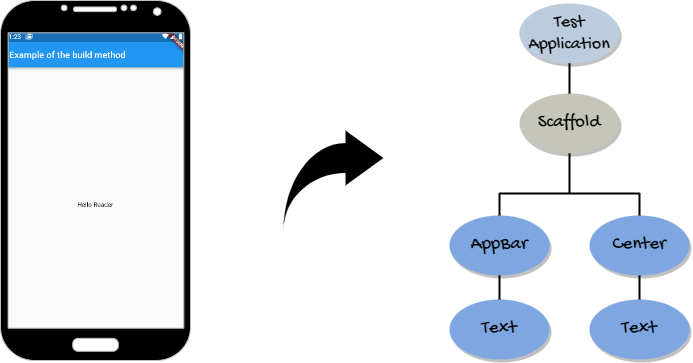
\includegraphics[scale=0.45]{widget_tree.png}
	\caption[Widget Tree of Listing 2.1]{Widget Tree of Listing 2.1}
\end{figure}
\subsection{Flutter: Architectural Layers}
A well-designed application architecture helps improve the system's performance, maintainability, and scalability and makes it more modular. [Buch: Software architecture seite 28] Many different application architectural patterns can be used, including the layered architecture Flutter uses. In software development, layered architecture is a typical design pattern in which the application is divided into different layers. Each layer plays a specific role in the overall functionality of the application. The Flutter architecture includes several critical components, including the Flutter engine, the Dart platform, and the Flutter framework. The Flutter engine renders widgets and manages their interactions with the underlying platform, such as the operating system and device hardware. The Dart platform provides the runtime environment for the Flutter app, including the Dart virtual machine (VM) and the core libraries. Application architecture refers to how the various components of a mobile or web application are organized and how they interact with each other. No layer has privileged access to the layers below, and every part of the framework layer is designed to be optional and interchangeable \cite{.flutterarchitecture}. Figure 3.2 shows the basic structure of a Flutter application. 
\begin{figure}[H]
	\centering
	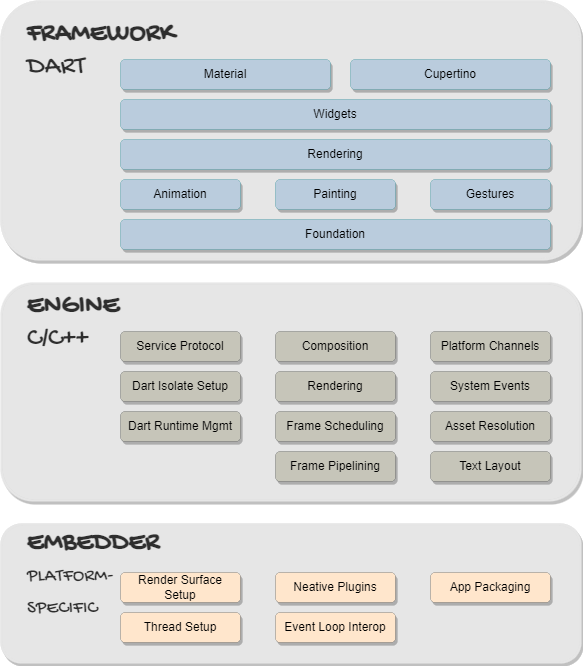
\includegraphics[scale=0.45]{layered_architecture.png}
	\caption[Layered Architecture in Flutter]{Layered Architecture in Flutter[based on \cite{.flutterarchitecture} and \cite[p. 50]{.flutterinaction}}
\end{figure}

\subsection{Programming Paradigm}
The programming paradigm of the Dart programming language is object-oriented programming (OOP). This means that it uses objects, classes, and inheritance to organize and structure code. Dart also incorporates some functional programming concepts, such as immutable data and first-class functions, which allow for more concise and elegant code. Additionally, Dart supports asynchronous programming, which enables developers to write code that can run concurrently and handle multiple tasks at the same time. Overall, Dart's combination of OOP and functional programming paradigms makes it a versatile and powerful language for building modern web and mobile applications. The SOLID principles are a set of guidelines for designing object-oriented software. They were introduced by Robert C. Martin in his book "Agile Software Development, Principles, Patterns, and Practices" as a way to improve the maintainability, extensibility, and flexibility of object-oriented code and to develop software that is prone to fewer bugs and has cleaner source code \cite{.martin}. These principles should be considered when developing the application.
\begin{itemize}
	\item \textbf{Single Responsibility Principle (SRP):}
	The SRP nstructs the developer to develop classes and software components so that they take on a maximum of one responsibility. In other words, a class should focus on a single task or piece of functionality and should not be responsible for multiple unrelated things. This helps reduce complexity and improve a software system's maintainability, testability, and extensibility. Another positive side-effect of this principle is that the written code is easier to understand, and error testing can be done more efficiently \cite{.martin}.
	
	\item \textbf{Open/Closed Principle (OCP):}
	According to the open-closed principle, software classes should be open for extension but closed for modification, which means a class should be designed to be easily extended or customized without changing its existing code. This allows developers to add new features or behaviors to a class without breaking its functionality. These classes or software components ought to be developed to allow other system entities to use their essential features without requiring access to the original entity's source code. 
	
	\item \textbf{Liskov Substitution Principle (LSP):}
	The Liskov Substitution Principle (LSP) asserts, in essence, that whenever a function uses a pointer or reference to a base object, it must also use a pointer or reference to any of its derived objects. [Software architecture with c++] It is also an extension of the OCP. A subclass should be able to be used wherever its superclass is expected without breaking the program's functionality. [stickify, solid design liskov] The Liskov Substitution Principle helps improve a software system's flexibility and reusability.
	
	\item \textbf{Interface Segregation Principle (ISP):}
	The Interface Segregation Principle ensures that clients of a class should not implement an interface containing methods that are irrelevant to its functionality. This helps to avoid creating large and complex interfaces that are difficult to implement and maintain. The Interface Segregation Principle promotes the creation of small, focused, and easy-to-use interfaces. 
	
	\item \textbf{Dependency Inversion Principle (DIP):}
	The fundamental essence of the DIP is that a class should not depend on the specific implementation details of another class. Instead, it should depend on an abstract interface or a set of contracts that define how the two classes should interact.
\end{itemize}



\section{NoSQL Databases}

\subsection{Introduction to NoSQL Databases}
The generic term NoSQL describes database systems that, unlike SQL databases, are not subject to the relational database model. The abbreviation NoSQL stands for "Not only SQL". The reasons why NoSQL databases have gained interest in recent years can be explained based on two aspects: In contrast to relational databases, which present their data storage in a table format, NoSQL databases benefit from different database models: document-oriented, key Value, graph, and column databases. This wide range of different data models allows developers to choose the model that best suits their application design. The result is a minimization of the code to be developed for an application. In addition, NoSQL databases allow administrators to scale their data on one machine and hardware clusters so that data volumes can be expanded without an expensive investment in new servers.
\begin{figure}[H]
	\centering
	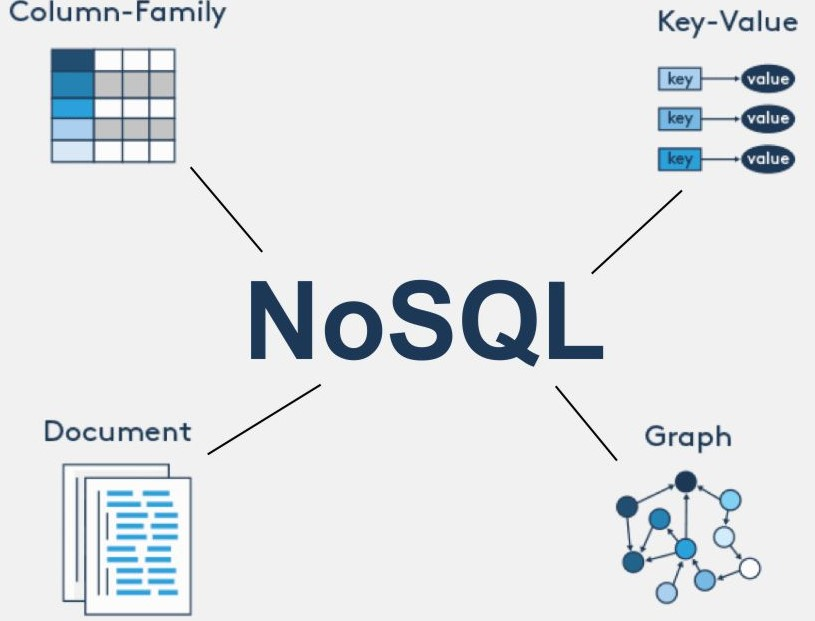
\includegraphics[scale=0.25]{nosql.jpg}
	\caption[NoSQL Data Models]{NoSQL Data Models}
\end{figure}

NoSQL databases support the use of CRUD operations.
\begin{itemize}
	\item \textbf{C:} create data
	\item \textbf{R:} read data
	\item \textbf{U:} update data
	\item \textbf{D:} delete data
\end{itemize}
The performance of some NoSQL databases even surpasses that of relational databases, especially with create and read operations. [Performance evaluation for CRUD] A detailed  performance comparison can be found in Appendix [Performance evaluation for CRUD].
\subsection{Firestore}
Cloud Firestore, more often called Google Firestore, is a cloud-hosted NoSQL database option that enables developers to store and synchronize their data in real-time, meaning that data that just got added to the database and changes made on already existing data is instantly shown to the application users. It is a part of Google's Backend-as-a-Service (BaaS) Firebase. BaaS is a concept where developers can use a platform to run their applications without managing servers and other infrastructure components. BaaS platforms offer various services required for applications, such as databases, authentication, storage, and APIs. [okta.com] To use BaaS, developers must first create an account with a BaaS platform and register their application. The platform then provides a set of APIs and SDKs that developers can use to access the services and integrate them into their applications. Most BaaS platforms offer a web-based console that developers can use to manage their applications and configure the services, and so does Firebase. Since Google publishes Firestore, it comes with peak reliability and excellent performance. Something worth mentioning is that Firestore can be used with far more programming languages than Dart and is also compatible with REST and RPC APIs. [firestorewebsite] Cloud Firestore caches data that your app is actively using, so the app can write, read, listen to, and query data even if the device is offline. When the device returns online, Cloud Firestore synchronizes any local changes to its servers.
\begin{lstlisting}[language=Python, caption={Dart - Firestore-Query}]
	
Future<DocumentSnapshot> checkCacheBeforeServer() async {
	try {
		DocumentSnapshot snapshot = await this.get(GetOptions(source: Source.cache));
		if (snapshot == null) return this.get(GetOptions(source: Source.server));
		return snapshot;
	} catch e {
		print(e);
		return this.get(GetOptions(source: Source.server));
	}
}
	
\end{lstlisting}
\noindent

\subsection{Document Databases}
There are several different NoSQL databases, which all rely on different data models. Firestore makes use of the document-based data format. This means that data stored in the database is accessible via collections filled with documents. For better understanding, one can imagine a collection in Firestore as a table in relational Databases, and a Document in Firestore equals a row in the relational schema. An example of that is shown in figure x.x. Documents in Firestore store their data in a key-value format, making it possible for a developer to store different documents in each collection. A quick view at an example makes this easier to understand: A developer wants to develop a restaurant-review application. For that, he created a collection named "restaurants" in firestore. Two of the three restaurants he now wants to add to the collection got a slogan with their brand, which he wants to add to the documents. The other restaurant does not have one. In a relational database, he still would have to fill the "slogan" column with at least NULL-data or an empty String (or whatever datatype the column has). Firestore, or document-based databases in general, allow it to just not add the slogan attribute to the third restaurant, which helps only to store relevant data to the database. One thing to remember is that even if the third restaurant gets a slogan one day, the developer can add that field to the document later. Cloud Firestore also stores subcollections or complex nested objects in documents. Firestore has no option to store foreign keys in a document.
